\section{Sistemas de Veículos Aéreos Não Tripulados}

    Esta seção fornece uma visão geral dos conceitos fundamentais necessários para compreender os sistemas de VANT, seus mecanismos de controle e os princípios de coordenação em enxames. Começamos detalhando os principais componentes e classificações dos VANTs, seguido por uma discussão sobre estratégias de controle e, por fim, as arquiteturas de enxames.

    \subsection{Principais componentes de um VANT}
        Um VANT (Veículo Aéreo Não Tripulado) consiste em diversos componentes essenciais que possibilitam sua operação autônoma. Estes incluem:
        \begin{itemize}
            \item \textbf{Estrutura do Drone:} O quadro (ou frame) de um drone é a estrutura física que serve como base para todos os seus componentes. Ele é responsável por suportar os motores, hélices, controladores de voo, baterias, sensores e demais módulos eletrônicos. Em geral, o frame é projetado para ser leve, rígido e resistente, a fim de garantir estabilidade e eficiência durante o voo.
            \item \textbf{Sistema de Propulsão:} Motores elétricos e hélices para UAVs de múltiplos rotores ou motores a combustão para drones de asa fixa de maior porte.
            \item \textbf{Controladora de Voo:}  É o componente central do drone responsável por interpretar os dados dos sensores (como giroscópios, acelerômetros, GPS e magnetômetros) e enviar comandos precisos aos motores para estabilizar e controlar o voo.
            \item \textbf{Computador embarcado:} Sistema de computação embarcada que realiza o processamento de dados oriundos dos sensores, do controlador de voô e da estação solo. Geralmente neste componente que ocorre a execução dos algoritmos de visão computacional essenciais para a navegação do drone. Neste componente que as decisões de alto nível são tomadas e repassadas à controladora de voo.
            \item \textbf{Sensores:} Unidades de Medição Inercial (IMU), GPS, LiDAR, câmeras e barômetros, que auxiliam na navegação, estabilidade e percepção do ambiente.
            \item \textbf{Sistema de Comunicação:} Links de dados para telemetria, controle e coordenação entre os agentes.
        \end{itemize}

        % Os UAVs podem ser classificados com base em:
        % \begin{enumerate}
        %     \item \textbf{Tamanho e Peso:} UAVs nano, micro, pequenos, médios e grandes.
        %     \item \textbf{Nível de Autonomia:} Drones pilotados remotamente, semiautônomos e totalmente autônomos.
        %     \item \textbf{Capacidades de Voo:} UAVs de asa fixa (maior autonomia), UAVs de rotores (capacidade de pairar) e UAVs híbridos.
        % \end{enumerate}

        %\noindent\textbf{TO-DO:} Criar Diagrama ilustrando os componentes que constituem um VANT, ou tirar foto do drone no Laboratorio

    \subsection{Dinâmica de Voo de um Quadricóptero}

        Neste trabalho, adota-se como plataforma aérea um veículo multirrotor com quatro motores, denominado quadricóptero (\textit{quadcopter}). Esse tipo de VANT apresenta seis graus de liberdade, sendo três translacionais e três rotacionais, associados aos movimentos de rolagem (\textit{roll}), arfagem (\textit{pitch}) e guinada (\textit{yaw}). A modelagem de sua dinâmica é fundamental para compreender a relação entre os comandos aplicados aos rotores e o movimento resultante do veículo.

        Considere o vetor $\boldsymbol{\omega} = [\omega_1, \omega_2, \omega_3, \omega_4]$, que representa as velocidades angulares dos quatro motores, e o vetor de ângulos de Euler $[\phi, \theta, \psi]$, correspondente à orientação do veículo no espaço. As forças e momentos gerados pelos rotores podem ser expressos pelas seguintes relações:

        \begin{align}
            u_f &= b(\omega_1^2 + \omega_2^2 + \omega_3^2 + \omega_4^2), \quad \text{[Empuxo total]},\\
            u_\phi &= bL(\omega_4^2 - \omega_2^2), \quad \text{[Momento de rolagem]}, \\
            u_\theta &= bL(\omega_3^2 - \omega_1^2), \quad \text{[Momento de arfagem]}, \\
            u_\psi &= d(\omega_1^2 - \omega_2^2 + \omega_3^2 - \omega_4^2), \quad \text{[Momento de guinada]},\\
            m\ddot{\mathbf{p}} &= -m\mathbf{g} + \mathbf{R}\,\mathbf{e}_3\,u_f, \quad \text{[Dinâmica translacional]}.
        \end{align}

        Nessas equações, $b$ representa o coeficiente de empuxo dos rotores, $d$ o coeficiente de arrasto aerodinâmico, $L$ a distância entre cada motor e o centro de massa do veículo, $\mathbf{R}$ a matriz de rotação do referencial do corpo para o referencial inercial, $\mathbf{e}_3 = [0,0,1]^\top$ o eixo $z$ do corpo, $m$ a massa total do VANT e $\mathbf{g}$ o vetor de aceleração gravitacional. Os sinais associados aos momentos dependem da convenção adotada para a numeração e o sentido de rotação dos motores.

        A dinâmica rotacional do quadricóptero pode ser descrita de forma compacta por:

        \begin{equation}
            \mathbf{I}\dot{\boldsymbol{\Omega}} + \boldsymbol{\Omega} \times (\mathbf{I}\boldsymbol{\Omega}) = \boldsymbol{\tau},
        \end{equation}

        em que $\boldsymbol{\Omega}$ representa o vetor de velocidades angulares do corpo, $\mathbf{I}$ a matriz de inércia e $\boldsymbol{\tau} = [u_\phi, u_\theta, u_\psi]^\top$ o vetor de momentos aplicados.

        A partir desse modelo, observa-se que o movimento do quadricóptero é obtido por meio da coordenação adequada das velocidades angulares dos rotores, permitindo a geração controlada de forças e momentos responsáveis tanto pela translação quanto pela orientação do veículo. Dessa forma, o sistema de controle de voo deve atuar diretamente sobre $\boldsymbol{\omega}$, de modo a garantir que a dinâmica resultante siga a trajetória e a atitude desejadas.

        \begin{figure}[H]
            \centering
            \includegraphics[scale=0.5]{fig/uav_dynamics_3.png}   
            \caption{Diagrama esquemático da dinâmica de um VANT com quatro motores.}
            \label{fig:dynamic_quadrotor}
        \end{figure}

    \subsection{Sistemas de Controle de Voo}
        %TODO verificar referencias e equacoes da dinamica do quadricoptero
        Um sistema de controle de voo de UAV é o mecanismo central que mantém e ajusta a orientação de um drone durante o voo, gerenciando o yaw, pitch e roll. Esse sistema de controle depende do feedback dos sensores para comparar continuamente a atitude real com o estado desejado, efetuando correções rápidas para garantir a estabilidade. Dentre as principais estratégias existente para o controle de voo, existem desde técnicas clássicas até métodos avançados baseados em IA. 

    \subsubsection*{\textbf{Controle Clássico Baseado em PID}}
        Os controladores PID nos sistemas de voo utilizam da teoria clássica de controle, especialmente na análise no domínio da frequência das funções de transferência. Ao representar o comportamento dinâmico do UAV por meio de uma função de transferência, é possível estudar como o sistema responde a diferentes frequências. O controlador PID ajusta os ganhos proporcional, integral e derivativo para modelar a resposta em frequência, aprimorando a estabilidade e o desempenho do sistema. Esse processo de ajuste garante que a atitude do drone — seu roll, pitch e yaw — permaneça responsiva aos comandos de controle, minimizando ultrapassagens e oscilações. Em essência, o projeto do controlador PID aproveita os insights matemáticos obtidos a partir da resposta em frequência do sistema, possibilitando uma estratégia de controle precisa e robusta para manter um desempenho de voo ideal.
        O sinal de controle de saída é matematicamente definido no domínio do tempo como:
        \begin{equation}
            u(t) = K_p \, e(t) + K_i \int_0^t e(\tau) \, d\tau + K_d \, \frac{d}{dt} e(t).
        \end{equation}
        onde:
        \begin{itemize}
            \item $u(t)$ é o comando de controle enviado aos atuadores.
            \item $e(t)$ é o erro entre o estado desejado e o real.
            \item $K_p$, $K_i$ e $K_d$ são os ganhos proporcional, integral e derivativo, respectivamente.
        \end{itemize}
        Aplicando a transformada de Laplace o sinal de controle torna-se:
        \begin{equation}
            C(s) = K_p + \frac{K_i}{s} + K_d s.
        \end{equation}
        \begin{figure}[H]
            \centering
        \begin{center}
        \begin{tikzpicture}[auto, node distance=1cm]

            % Nodes
            \node [sum] (sum) {$+$};
        \node [block, right=of sum] (controller) {$C(s) = K_p + \frac{K_i}{s} + K_d s$};
            \node [block, right=of controller] (quad) {$G(s) = \frac{1}{I s^2}$};
            \node [coordinate, right=of quad] (output) {};
            \node [coordinate, below=1.5cm of quad] (feedback) {};
            \node [coordinate, left=of sum] (input) {};

            % Arrows
            \draw [arrow] (input) -- node{\Large$R(s)$} (sum);
            \draw [arrow] (sum) -- (controller);
            \draw [arrow] (controller) -- node{\Large$u(t)$} (quad);
            \draw [arrow] (quad) -- node{\Large$Y(s)$} (output);
            \draw [arrow] (output) |- (feedback) -| node[pos=0.9, above]{\Large$-$} (sum);

        \end{tikzpicture}
        \end{center}
            \caption{Malha de controle fechada quadrotor.}
            \fonte{Elaborado pelo autor.}
            \label{fig:malha_fechada_drone}
        \end{figure}
        Em que $G(s)$ representa a função transferência de malha aberta que modela a dinâmica do drone com 4 rotores, sendo $I$  momento de inércia sob os respectivos eixos. $R(s)$ indica a entrada de referência, ou seja, os ângulos roll, pitch e yaw desejados. $Y(s)$ representa a saída obtida a partir dos sensores IMU do drone, que são retroalimentados para computação do erro, ajustando a entrada do controlador.

        %\noindent\textbf{Sugestão de Ilustração:} Diagrama em blocos de um sistema de controle de voo de UAV usando PID, mostrando comandos de entrada, loops de feedback e resposta dos atuadores.


        
%%%%%% ######## Enxame de VANTs ########%%%%%%
    
\section{Enxames de Veículos Aéreos Não Tripulados}
    \subsection{Definição }
        Um \textbf{enxame de veículos aéreos não tripulados (VANTs)} refere-se a um conjunto de drones autônomos ou semiautônomos que operam de forma cooperativa e distribuída com o objetivo de cumprir uma missão comum. Esse paradigma é fortemente inspirado em comportamentos coletivos observados na natureza, como colônias de insetos sociais, e caracteriza-se por propriedades como robustez, flexibilidade e eficiência operacional. Estudos clássicos, como os de \citeonline{brambilla2013swarm} e \citeonline{chung2018survey}, consolidaram esse conceito no contexto da robótica móvel e aérea.

        Entre as principais propriedades que caracterizam um enxame de VANTs, destacam-se:
        \begin{itemize}
            \item \textbf{Arquitetura}: define a forma como as decisões são tomadas e distribuídas entre os agentes, podendo assumir configurações centralizadas, descentralizadas ou híbridas, conforme a taxonomia apresentada por \citeonline{bayndir2016review}.
            \item \textbf{Escalabilidade}: capacidade do sistema de manter desempenho adequado à medida que o número de agentes aumenta, aspecto fundamental para operações com dezenas ou centenas de VANTs \cite{chung2018survey}.
            \item \textbf{Adaptabilidade}: habilidade do enxame de reagir a mudanças no ambiente, como obstáculos, alvos móveis ou novas missões, sendo essencial em cenários dinâmicos e não estruturados, conforme discutido por \citeonline{ollero2021past}.
            \item \textbf{Redundância}: tolerância a falhas obtida pela distribuição de funções entre múltiplos agentes, permitindo a continuidade da missão mesmo diante da perda de um ou mais VANTs.
        \end{itemize}

    \subsection{Arquiteturas de Enxames}

        As arquiteturas de controle de enxames de VANTs podem ser classificadas em três categorias principais: centralizada, descentralizada e híbrida, de acordo com o grau de distribuição do processo decisório.

        Na \textbf{arquitetura centralizada} (Figura~\ref{fig:arquitetura_central}), um nó controlador central, geralmente representado por uma estação solo, é responsável por coletar informações dos VANTs e emitir comandos de controle. Essa abordagem facilita a coordenação global e possibilita a execução de otimizações centralizadas. Contudo, apresenta limitações significativas, como baixa escalabilidade e a presença de um ponto único de falha, tornando-se inadequada para missões em larga escala ou ambientes com conectividade instável.

        A \textbf{arquitetura descentralizada} (Figura~\ref{fig:arquitetura_desc}) distribui a tomada de decisão entre os próprios VANTs, que atuam com base em observações locais e comunicação entre pares. Nessa configuração, cada agente deve possuir maior autonomia, frequentemente viabilizada por algoritmos de inteligência artificial. Essa abordagem apresenta elevada robustez e escalabilidade, porém impõe desafios adicionais de coordenação e pode resultar em soluções subótimas quando comparada a abordagens centralizadas.

        Por fim, a \textbf{arquitetura híbrida} (Figura~\ref{fig:arquitetura_hibrida}) combina elementos das duas abordagens anteriores. Um componente central é responsável pelo planejamento de alto nível, como a atribuição de tarefas, enquanto a execução ocorre de forma descentralizada entre os VANTs. Essa configuração busca equilibrar controle global e autonomia local, oferecendo maior flexibilidade e resiliência operacional.

        \begin{figure}[h]
            \centering
            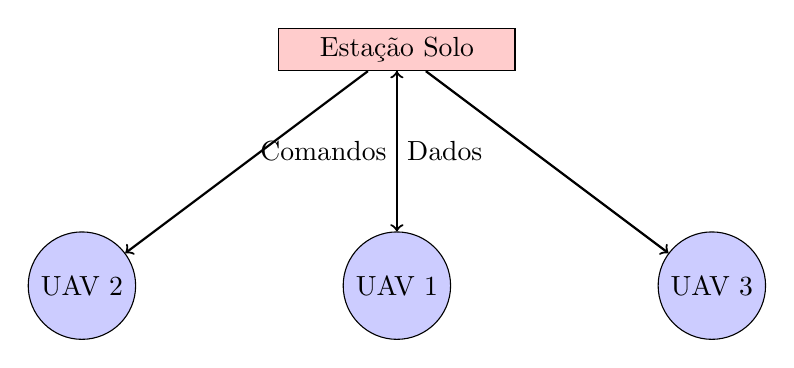
\begin{tikzpicture}[node distance=2cm]
            % Controlador Central
            \node[draw, rectangle, fill=red!20, minimum width=3cm] (central) {Estação Solo};
            % UAVs
            \node[draw, circle, fill=blue!20, below of=central, yshift=-1cm] (uav1) {UAV 1};  
            \node[draw, circle, fill=blue!20, left of=uav1, xshift=-2cm] (uav2) {UAV 2};  
            \node[draw, circle, fill=blue!20, right of=uav1, xshift=2cm] (uav3) {UAV 3};  
            % Conexões
            \draw[->, thick] (central) -- (uav1) node[midway, left] {Comandos};  
            \draw[->, thick] (central) -- (uav2);  
            \draw[->, thick] (central) -- (uav3);  
            \draw[->, thick, dashed] (uav1) -- (central) node[midway, right] {Dados};  
        \end{tikzpicture}
            \caption{Arquitetura Centralizada.}
            \fonte{Elaborado pelo autor.}
            \label{fig:arquitetura_central}
        \end{figure}

        \begin{figure}[h]
            \centering
            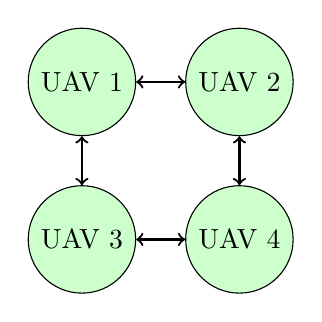
\begin{tikzpicture}[node distance=2cm]
            % UAVs
            \node[draw, circle, fill=green!20] (uav1) {UAV 1};  
            \node[draw, circle, fill=green!20, right of=uav1] (uav2) {UAV 2};  
            \node[draw, circle, fill=green!20, below of=uav1] (uav3) {UAV 3};  
            \node[draw, circle, fill=green!20, below of=uav2] (uav4) {UAV 4};  
            
            % Conexões peer-to-peer
            \draw[<->, thick] (uav1) -- (uav2);  
            \draw[<->, thick] (uav1) -- (uav3);  
            \draw[<->, thick] (uav2) -- (uav4);  
            \draw[<->, thick] (uav3) -- (uav4);  
        \end{tikzpicture}
            \caption{Arquitetura Descentralizada.}
            \label{fig:arquitetura_desc}
        \end{figure}


        \begin{figure}[h]
            \centering
            \begin{tikzpicture}[node distance=3cm]
            % Central Planner
            \node[draw, rectangle, fill=orange!20] (central) {Estação Solo};
            % Subgroup Leaders
            \node[draw, diamond, fill=purple!20, below left of=central] (lider1) {Lider 1};  
            \node[draw, diamond, fill=purple!20, below right of=central] (lider2) {Lider 2};  
            % Planner connections
            \draw[->, dashed, thick] (central) -- (lider1);  
            \draw[->, dashed, thick] (central) -- (lider2);  
            % Subgroups
            \node[draw, circle, fill=cyan!20, below left of=lider1] (uav1) {UAV A};  
            \node[draw, circle, fill=cyan!20, right of=uav1] (uav2) {UAV B};
            \node[draw, circle, fill=cyan!20, right of=uav2] (uav3) {UAV C};  
            \node[draw, circle, fill=cyan!20, below right of=lider2] (uav4) {UAV D};  
            %\node[draw, circle, fill=cyan!20, left of=uav4] (uav5) {UAV E};  
            % Peer-to-peer connections
            \draw[<->, thick] (lider1) -- (uav1); 
            \draw[<->, thick] (lider1) -- (uav2);  
            \draw[<->, thick] (uav1) -- (uav2);  
            \draw[<->, thick] (lider2) -- (uav3);  
            \draw[<->, thick] (lider2) -- (uav4);
            \draw[<->, thick] (uav3) -- (uav4);
            \draw[<->, thick] (uav2) -- (uav3);  
        \end{tikzpicture}
            \caption{Arquitetura Híbrida.}
            \fonte{Elaborado pelo autor.}
            \label{fig:arquitetura_hibrida}
        \end{figure}


    \subsection{Aplicações e Comportamentos de Enxames de VANTs}

        Os enxames de VANTs têm sido amplamente explorados em diferentes domínios devido à sua capacidade de realizar missões cooperativas de forma eficiente e escalável. Entre as principais aplicações, destacam-se tarefas de vigilância e reconhecimento, como patrulhamento de fronteiras e rastreamento de alvos, nas quais múltiplos VANTs podem cobrir grandes áreas simultaneamente. Em cenários de resposta a desastres, esses sistemas são empregados em operações de busca e resgate e avaliação de danos, permitindo atuação segura em ambientes de difícil acesso.

        Na agricultura de precisão, enxames de VANTs são utilizados para monitoramento de culturas, detecção de pragas e pulverização seletiva, enquanto em contextos de comunicação podem atuar como redes móveis temporárias para fornecer conectividade em áreas remotas ou durante emergências. Em aplicações militares, esses sistemas são empregados em missões coordenadas de reconhecimento, guerra eletrônica e operações ofensivas, explorando sua adaptabilidade e redundância.

        A execução eficiente dessas aplicações depende de um conjunto de \textbf{comportamentos coletivos} característicos dos sistemas de enxame. Dentre eles, destacam-se a formação de voo, que permite a manutenção de padrões geométricos organizados; a alocação dinâmica de tarefas entre os agentes; o planejamento colaborativo de trajetórias e desvio de obstáculos; a tomada de decisão coletiva; e a autorreconfiguração do enxame diante de falhas ou perdas de agentes. Esses comportamentos emergem da interação local entre os VANTs e são fundamentais para a robustez e flexibilidade do sistema.


    
    \subsection{Principais Desafios no Controle de Enxames de VANTs}
        Apesar de suas vantagens, o controle de enxames de VANTs envolve diversos desafios técnicos e operacionais, especialmente em ambientes reais e dinâmicos. A Tabela~\ref{tab:desafios_enxame} sintetiza os principais desafios associados a esse problema.

        \begin{table}[H]
        \centering
        \caption{Principais desafios no controle de enxames de VANTs}
        \label{tab:desafios_enxame}
        \begin{tabular}{p{4cm} p{10cm}}
        \toprule
        \textbf{Desafio} & \textbf{Descrição} \\
        \midrule
        Não estacionariedade &
        A presença de múltiplos agentes aprendendo ou tomando decisões simultaneamente altera continuamente a dinâmica do ambiente percebido por cada VANT. \\

        Observabilidade parcial &
        Cada agente possui acesso limitado ao estado global do sistema, dificultando a coordenação e a tomada de decisões cooperativas. \\

        Escalabilidade &
        O aumento do número de VANTs eleva os custos computacionais e de comunicação, dificultando o controle eficiente do enxame. \\

        Ambientes dinâmicos &
        Mudanças no ambiente, obstáculos móveis e alvos dinâmicos exigem adaptação e replanejamento em tempo real. \\

        Restrições físicas &
        Limitações de autonomia energética, capacidade computacional embarcada e precisão de sensores e atuadores. \\

        Segurança e resiliência &
        Vulnerabilidade a falhas, interferências eletromagnéticas e ataques cibernéticos, além da presença de agentes adversários. \\
        \bottomrule
        \end{tabular}
        \end{table}

        Esses desafios evidenciam a necessidade de abordagens avançadas de controle e coordenação, motivando o uso de técnicas de aprendizado por reforço multiagente e arquiteturas distribuídas capazes de lidar com ambientes complexos, dinâmicos e parcialmente observáveis.
